\documentclass[9pt,twocolumn,twoside]{osajnl}

\journal{jocn} 

% See template introduction for guidance on setting shortarticle option
\setboolean{shortarticle}{false}
% true = letter / tutorial
% false = research / review article
% (depending on journal).

\title{\LaTeX\  Simulazione di un filtro digitale per la rilevazione di segnali neurali \emph{ }}

\author[1]{Alfredo Guarnieri}
% \author[2,*]{Author Two}
% \author[1]{Author Three}

% \affil[1]{Publications Department, The Optical Society (OSA), 2010 Massachusetts Avenue NW, Washington D.C., 20036, USA}
% \affil[2]{School of Science, University of Technology, 2000 J St. NW, Washington DC, 20036, USA}
% \affil[3]{School of Optics, University of Technology, 2000 J St. NW, Washington DC, 20036, USA}

% \affil[*]{Corresponding author: email@my-email.com}

%% To be edited by editor
% \dates{Compiled \today}

%\ociscodes{(140.3490) Lasers, distributed feedback; (060.2420) Fibers, polarization-maintaining;(060.3735) Fiber Bragg gratings.}

%% To be edited by editor
% \doi{\url{http://dx.doi.org/10.1364/XX.XX.XXXXXX}}

\begin{abstract}
Le proprietà spettrali di segnali rumorosi di impulsi in tensione caratterizzati da spaziatura e ritardo temporale irregolari, sono utilizzate in questo lavoro con l'intento di simulare un segnale di natura biologica e verificare le capacità predittive di alcuni test di soglia ampiamente utilizzati per la rilevazione di segnali provenienti da popolazioni di neuroni con tecnologia $MEA$, \cite{Lambacher2011}, \cite{Vallicelli2017}. 

L'analisi è condotta parallelamente sotto il profilo spaziale e temporale analizzando la distribuzione congiunta di, (1) una metrica spettrale per la distanza del segnale filtrato da quello originale e (2) un indice di precisione della rilevazione nel tempo degli impulsi.

Si conclude che i test di soglia in potenza accoppiati con filtri passa banda possono condurre a risultati imprecisi in merito alla rilevazione del tempo degli impulsi a causa delle distorsioni spettrali introdotte, sia per l'elevata rumorosità del segnale, che per l'ignota forma degli impulsi. Gli algoritmi di sorting a media semplice risultano invece più robusti e accurati, facendo leva solo sull'elevata frequenza di campionamento spazio-temporale.
\end{abstract}

% \setboolean{displaycopyright}{true}

\begin{document}

\maketitle



\section{Introduzione}

Nei contesti sperimentali di rilevazione di segnali neurali con tecnologia $MEA$ un segnale fortemente rumoroso nasconde degli impulsi in tensione di forma non nota che si manifestano in tempi non noti, con frequenza media
({\it mean spike rate}) dell'ordine di qualche $kHz$. Le capacità discriminanti di alcuni algoritmi di sorting del segnale proposti in letteratura
\cite{Vallicelli2017}, \cite{Lambacher2011} vengono  qui confrontati su un segnale di prova.

La simulazione introduce nel segnale di prova tre tipi di irregolarità suggerite sia dal contesto sperimentale di rilevazione del segnale, che dalla sua natura biologica: (1) rumore termico additivo; (2) intervalli di tempo casuali tra due impulsi successivi; (3) ritardo di fase di campionamento dell'impulso casuale.

Le variabili di simulazione riguardano le seguenti proprietà: (1) la distribuzione di probabilità dei tempi d'attesa tra due impulsi; (2) la forma degli impulsi; (3) lo spike rate medio; (4) SNR. Con riguardo alla prima le analisi preliminari hanno evidenziano che l'emersione dei picchi alla frequenza dello spike rate medio avviene solo quando la deviazione standard della distribuzione dei tempi d'attesa è sufficientemente bassa, è necessario quindi modellare tale distribuzione con almeno due parametri distinti, uno per la media e uno per la varianza. Sono state perciò scartate le più semplici distribuzioni di probabilità come quella rettangolare e quella del decadimento esponenziale\footnote{Note nella letteratura statistica rispettivamente come uniforme ed esponenziale negativa}. La varianza di tali distribuzioni è infatti funzionalmente dipendente dalla media e per la presente applicazione, troppo elevata. La distribuzione utilizzata è invece la distribuzione gamma, controllata da due parametri, uno di forma, detto $\lambda$ e uno di scala, detto $\beta$. La distribuzione gamma è la più semplice generalizzazione della distribuzione esponenziale negativa, potendosi ottenere come distribuzione della somma di un numero $\beta$ di variabili casuali esponenziali negative, tutte identicamente distribuite con parametro di media $\lambda$. In funzione di questi parametri lo spike rate medio è $\beta\lambda^{-1}$ e la varianza $\beta\lambda^{-2}$, in questo modo, variando opportunamente i due parametri $\lambda$ e $\beta$, si ottengono tutte le possibili configurazione dei primi due momenti dello spike rate. Con riguardo alla forma degli impulsi, l'analisi preliminare ha evidenziato una certa variabilità dei risultati, tale variabile di simulazione viene perciò conservata e sono stati proposti quattro tipi di impusi. Infine, con riguardo allo spike rate medio, i risultati preliminari non hanno dimostrato sufficiente variabilità in un ampio intervallo di frequenze a partire da qualche decina di $Hz$ fino al limite di $10kHz$, oltre il quale impulsi della durata di $1ms$ iniziano a sovrapporsi.

I test presi in considerazione dalla simulazione sono due, il primo proposto in letteratura da \cite{Lambacher2011}, è un test in potenza basato sulla media quadratica del segnale. Il secondo test, più semplice, utilizza la media aritmetica. Ognuno dei due test è variato con due diversi filtri in frequenza preliminari, un passa banda e un passa basso, applicati alternativamente per un totale di quattro test. 

Le conclusioni della simulazioni si basano sull'accuratezza delle capacità discriminanti dei due algoritmi di sorting. Nella fase preliminare dell'analisi, l'andamento congiunto di due metriche, una afferente al dominio delle frequenze e una al dominio dei tempi, mostra evidenze importanti a favore dei test a media artimentica, evidenza corroborata da un coerente andamento delle metriche al variare di tutte le variabili di simulazione.

Per trarre evidenze analitiche più precise, si propone infine un'analisi di classificazione delle previsioni dei due algoritmi di sorting, che viene riportata in misura media al variare di tutte le variabili di simulazione e per la ripetizione della simulazione su $100$ iterazioni, al fine di ottenere risultati più robusti con riguardo anche alle casualità introdotte. I risultati di simulazione vengono riassunti in quattro categorie: falsi positivi, veri positivi, falsi negativi e veri negativi. Le conclusioni si affidano a due indici di concordanza, l'indice di concordanza di Jaccard e il punteggio $F1$, noti nella letteratura in ambito di {\it data science} e ampiamente utilizzati per riportare l'accuratezza degli algoritmi di classificazione. Tali indici, sono in sostanza delle misure di correlazione, anche se trattandosi di variabili dicotomiche è corretto parlare di associazione o concordanza, tra la previsione dei tempi degli impulsi e i tempi effettivi, e sono, per comodità, uniformati a variare tra il valore $0$, che indica assenza di correlazione e $1$, massima dipendenza. 

I valori degli indici per i filtri a media aritmetica risultanti dalla presente simulazione sono sempre sensibilmente superiori a quelli degli algoritmi a media quadratica, indipendentemente dal tipo di filtro in frequenza applicato.



% This  template is designed to assist with creating an article to submit to the \emph{Journal of Optical Communications and Networking}. See the OSA's \href{http://www.opticsinfobase.org/submit/style/}{Style Guide} and \href{http://www.opticsinfobase.org/submit/templates/}{Manuscript Templates} pages for more details.
% 
% If you have a question while using this template on {Overleaf}, please use the help menu (``?'') on the top bar to search for help or ask us a question using our \href{https://www.overleaf.com/contact}{contact form}.



\section{Simulazione}
\label{sec:examples}

La seguente tabella \ref{tab:param} mostra i principali parametri di simulazione.

\begin{table}[htbp]
\centering
\caption{\bf Parametri di simulazione}
\begin{tabular}{ccc}
\hline
Durata segnale                  & 1s                \\
Spike rate (media)              & 150Hz             \\
Spike rate (errore standard)    & 0.01              \\
Durata spike                    & 1ms               \\
Ampiezza Max 0p                 & 60mV              \\
Potenza media spike            & 1.8$\mu V^{2}s$   \\
Campionamento                   & 9kSamples         \\
Filtro. $\nu_{low}$             & 0.02 kHz          \\
Filtro. $\nu_{high}$            & 2.5 kHz           \\
Pixels                          & 7                 \\
\hline
\end{tabular}
\label{tab:param}
\end{table}



\subsection{Impulsi e SNR}

Il segnale di prova è un treno di impulsi uniformemente distribuiti lungo la durata del segnale $T$. Ogni impulso $I(t'), t'\in[0,t]$ è campionamento a intervalli costanti con una fase casuale $\phi_{\mu}$, dove $\mu$ è il tempo casuale in cui si manifesta l'impulso.
%
\begin{align*}
 s_{n} &= \epsilon_{n} + I(k_{n} + \phi_{\mu})(\theta_{\mu+N} - \theta_{\mu})    \\
 \epsilon_{n} & \sim N(0,\sigma^{2}_{\epsilon})   \\
 \phi & \sim U(0,t), \quad\quad \mu  \sim  U(0,T )
\end{align*}
%
Gli impulsi considerati hanno uguale durata media e potenza trasferita e si distinguono per la forma (gaussiana, rettangolare, sinusoidale, ... ). Al tasso di campionamento considerato, ogni impulso è campionato per circa $N = 9kSamples/s (1ms) \simeq 9$ volte.

La potenza di rumore utilizzata per dato $SNR$ è stata calcolata tenendo conto della potenza trasferita nel tempo di durata di un singolo impulso, secondo le seguenti relazioni.
\begin{align*}
P_{noise} \quad [V^2s] &=  P_{impulse} 10^{- snr [dB]/10} \\
\sigma^{2}_{\epsilon} &= \frac{ P_{noise} }{ N }
\end{align*}
Con riferimento all'impulso di riferimento sinusoidale, il seguente grafico \ref{fig:c6_graphSNR} riporta le deviazioni standard utilizzate in funzione dell'$SNR$.
%
% \begin{figure}[htbp]
% \centering
% \fbox{\includegraphics[width=.5\linewidth]{results/c6_graphSNR.eps}}
% \caption{Varianza errore termico e $SNR$.}
% \label{fig:results/c6_graphSNR}
% \end{figure}



\subsection{Algoritmi di sorting}

La tabella \ref{tab:shapefunctions} mostra gli algoritmi di sorting analizzati.
I due algoritmi di base differiscono per l'ordine della media, aritmetica o quadratica. In entrambi compare il passaggio di media spaziale sui pixel che rilevano un singolo neurone. L'algoritmo a media quadratica riporta un ulteriore media temporale di ordine $3$. Ognuno dei due algoritmi viene implementato dopo l'applcazione di un filtro in frequenza che può essere, passa basso o passa banda alla frequenze indicate nella tabella \ref{tab:param}, per un totale di $4$ combinazioni.


\begin{algorithm}
\caption{Algoritmo lineare}\label{alg:arit}
\begin{algorithmic}[1]
%\Procedure{Euclid}{$a,b$}\Comment{The g.c.d. of a and b}
\State $s_{j,t}$ \Comment{Segnale al tempo t, pixel j}
\State $f_{j,t}$ \Comment{Filtro passa basso o passa banda}
\State $f_{t}\gets \sum_{1:7}   f_{j,t}/7$
\State $f_{t}\gets \sum_{i=1:3} f_{t-i}/3$
% \EndWhile\label{euclidendwhile}
% \State \textbf{return} $b$\Comment{The gcd is b}
% \EndProcedure
\end{algorithmic}
\end{algorithm}


\begin{algorithm}
\caption{Algoritmo quadratico}\label{alg:quad}
\begin{algorithmic}[1]
%\Procedure{Euclid}{$a,b$}\Comment{The g.c.d. of a and b}
\State $s_{j,t}$ \Comment{Segnale al tempo t, pixel j}
%\While{$r\not=0$}\Comment{We have the answer if r is 0}
\State $f_{j,t}$ \Comment{Filtro passa basso o passa banda}
\State $F_{j,t}\gets f^{2}_{j,t}$
\State $F_{t}\gets \sum_{1:7}   F_{j,t}/7$
\State $F_{t}\gets \sum_{i=1:3} F_{t-i}/3$
% \EndWhile\label{euclidendwhile}
% \State \textbf{return} $b$\Comment{The gcd is b}
% \EndProcedure
\end{algorithmic}
\end{algorithm}





\subsection{Sorting: profilo spettrale}

Le figure \ref{fig:c9_I5SNR4spec} e \ref{fig:c9_I2SNR4spec} mostrano l'effetto spettrale degli algoritmi su due segnali di prova.



\begin{figure}[htbp]
\centering
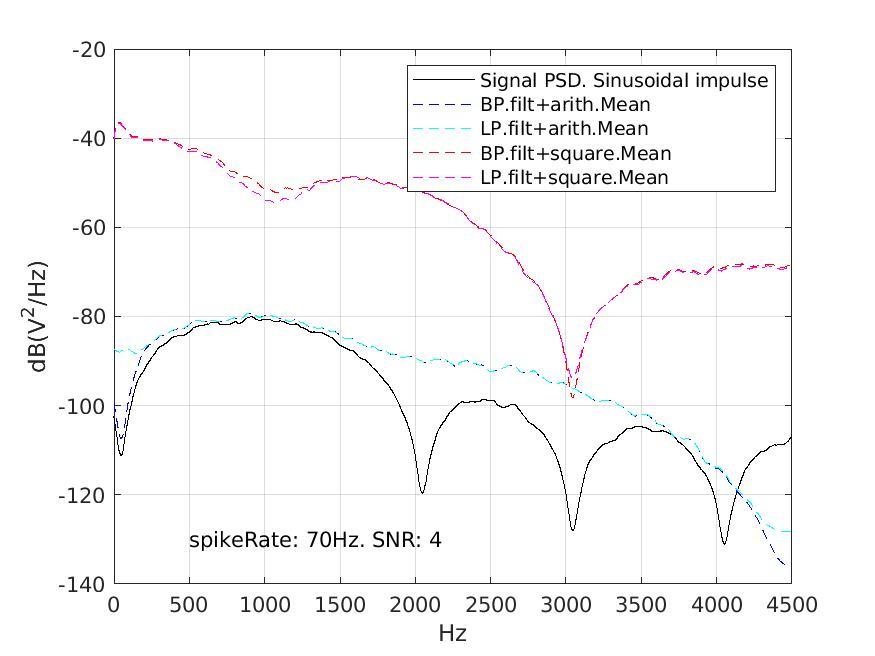
\includegraphics[width=1\linewidth]{results/c9_I5SNR4spec.jpg}
\caption{$SNR = 4dB$. PSDs}
\label{fig:c9_I5SNR4spec}
\end{figure}

Per entrambi i tipi di impulso considerato, l'algoritmo a media quadratica ha l'effetto di innalzare considerevolmente le basse frequenze. Si tratta di un {\it red shift} dovuto all'operazione di elevamente al quadrato accoppiato a (1) rumorosità del segnale: il quadrato di un segnale rumoroso sviluppa una componente in continua che si allarga anche alle basse frequenze. (2) Non linearità della trasformazione: con la qudratura compaiono frequenze fittizie che sono frutto di combinazioni lineari di quelle preesistenti nel segnale originale.

\begin{figure}[htbp]
\centering
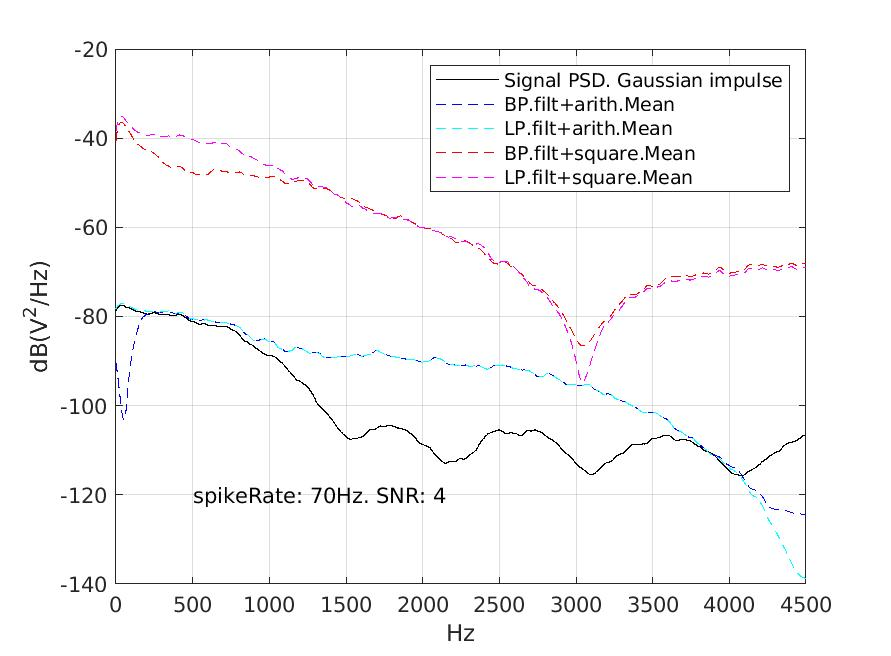
\includegraphics[width=1\linewidth]{results/c9_I2SNR4spec.jpg}
\caption{$SNR = 4dB$. PSDs.}
\label{fig:c9_I2SNR4spec}
\end{figure}

L'effetto di {\it red shift} è particolarmente dannoso per gli impulsi come quello sinusoidale dove la densità di potenza sulle basse frequenze dello spettro non rumoroso è molto bassa. Nel caso invece degli impulsi rettangoalre e gaussiano la forma dello spettro risulta meglio approssimata.




\section{Sorting: profilo temporale}

I seguenti grafici \ref{fig:c1_I2SNR0time} e \ref{fig:c1_I4SNR0time} mostrano la serie temporale del segnale di prova a $0dB$ e a confronto il segnale filtrato.


\begin{figure}[htbp]
\centering
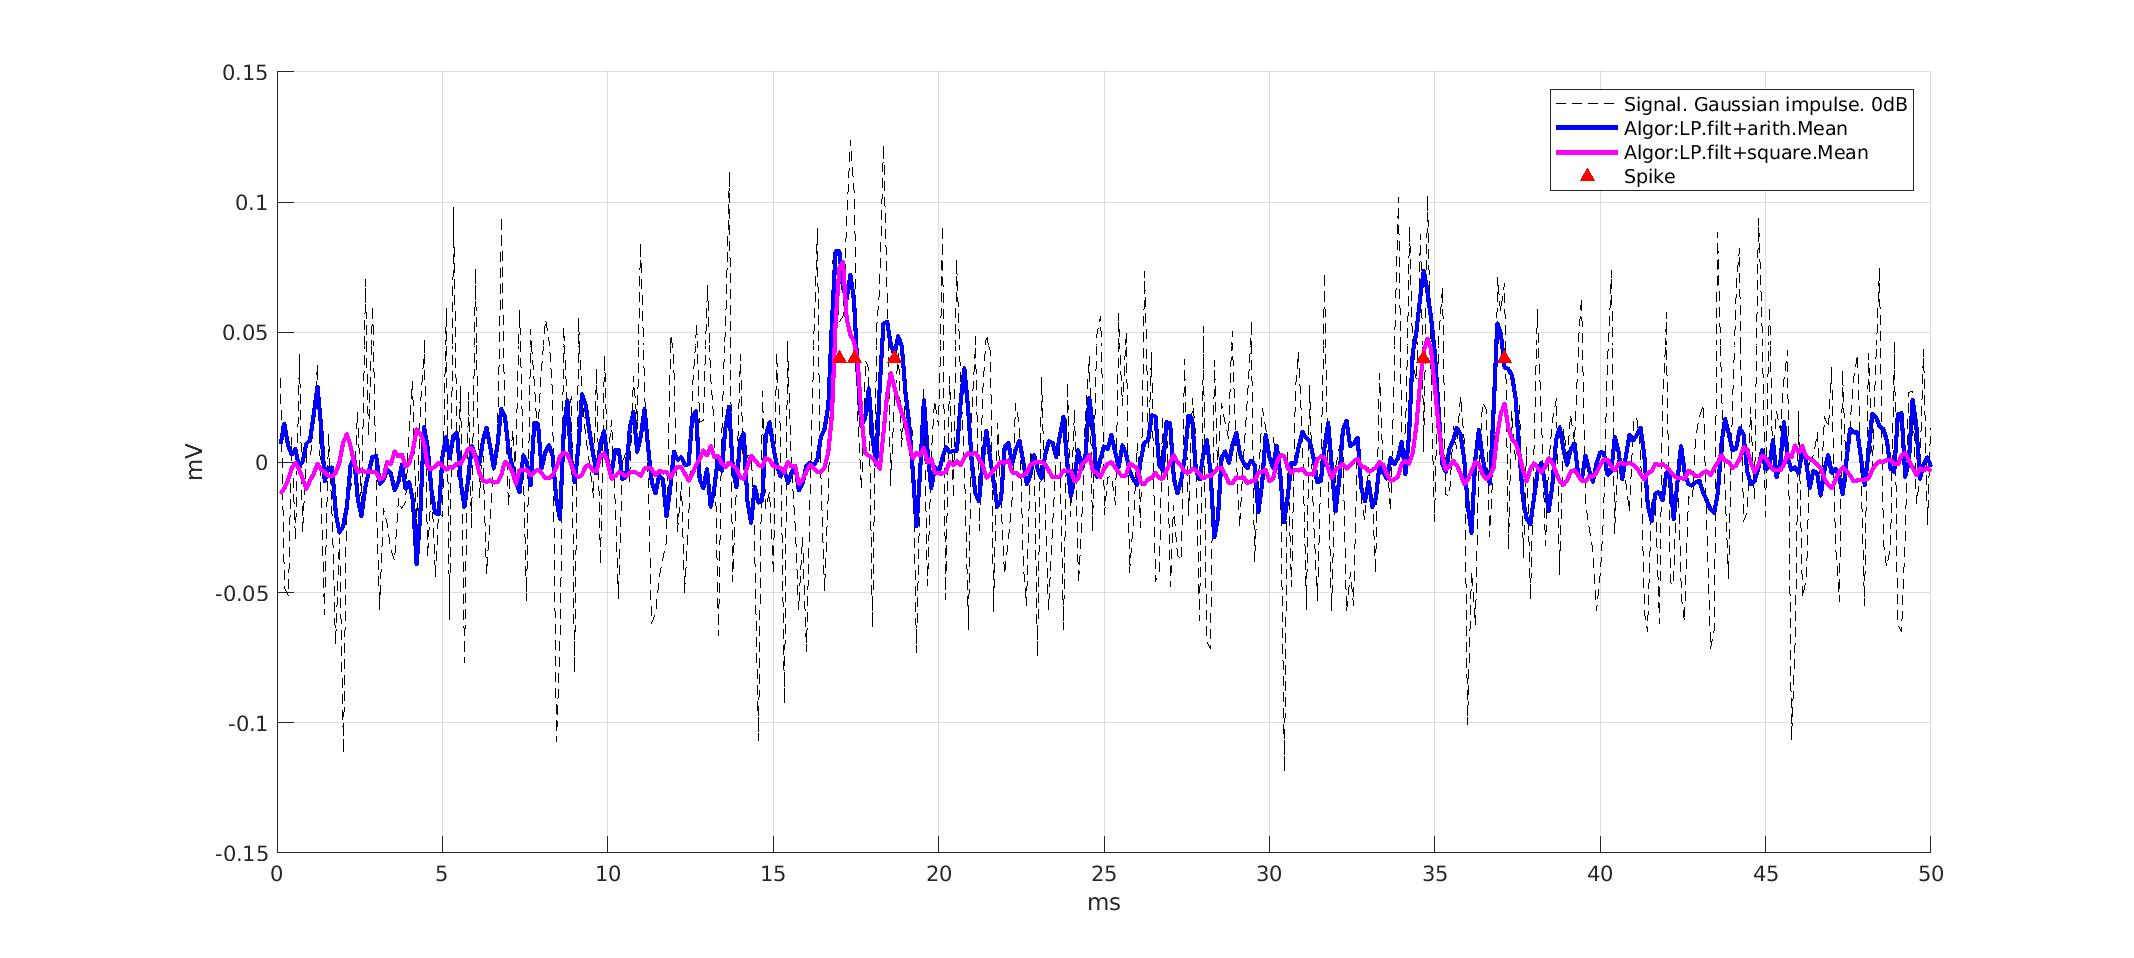
\includegraphics[width=1\linewidth]{results/c1_I2SNR0time.jpg}
\caption{Serie temporali. Segnale e filtri. Impulso gaussiano}
\label{fig:c1_I2SNR0time}
\end{figure}

\begin{figure}[htbp]
\centering
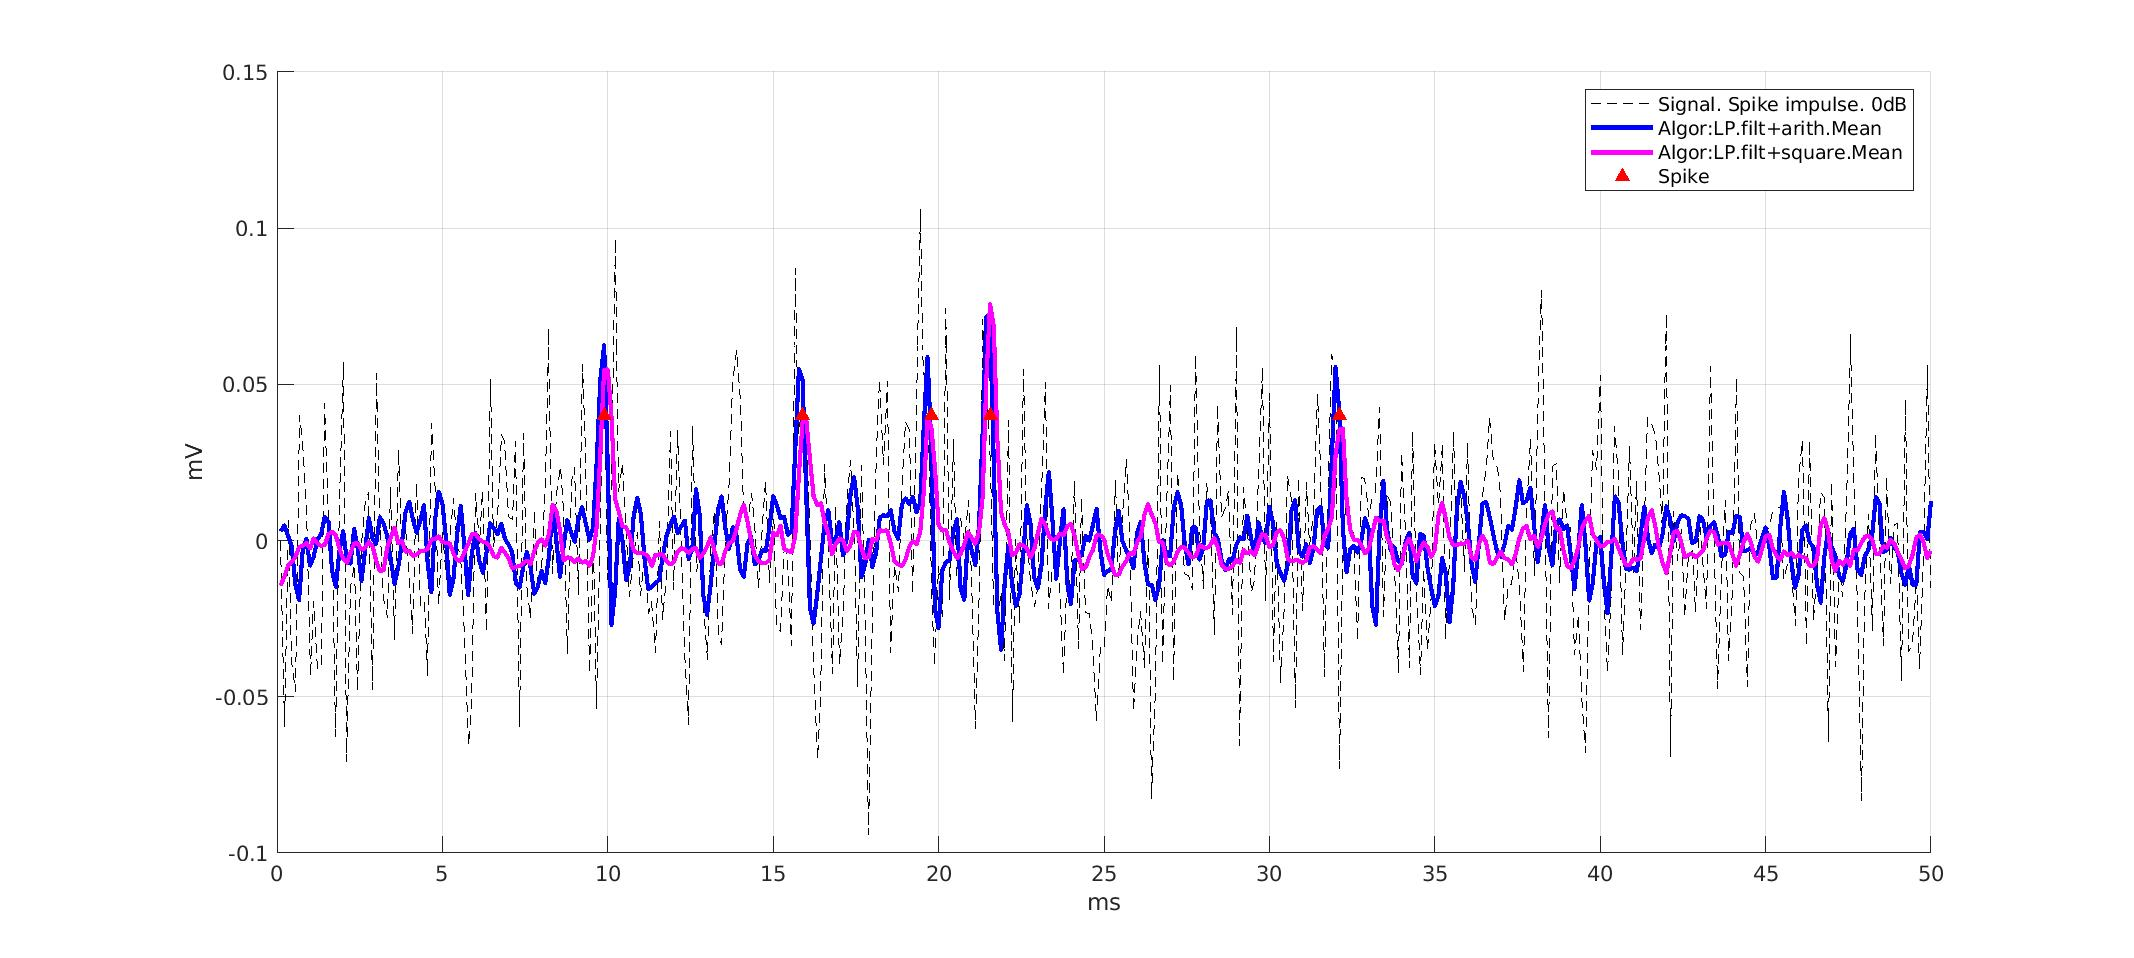
\includegraphics[width=1\linewidth]{results/c1_I4SNR0time.jpg}
\caption{Serie temporali. Segnale e filtri. Impulso spike}
\label{fig:c1_I4SNR0time}
\end{figure}




\section{Metriche di valutazione degli algoritmi}

Sotto il profilo spettrale un buon algoritmo di sorting trasforma uno spettro rumoroso in modo da ben approssimare i picchi delle frequenza caratteristiche del segnale non rumoroso (toni). Nel contesto di segnali ad impulsi irregolari, questo è ancora vero se si sostiutisce la visione tonica con una timbrica, in cui lo spettro non rumoroso non è composto da una serie di picchi in frequenza ma piuttosto da una forma caratteristica che riflette sia la forma degli impulsi sia l'irregolarità con cui essi appaiono nel segnale.

Con il fine di definire di quantificare l'approssimazione raggiunta da un algoritmo di sorting si propone una metrica per la distanza spettrale adottata in questo lavoro, paragrafo \ref{metricaS}.

Sotto il profilo temporale un buon algoritmo di sorting azzera il segnale dove non rileva impulsi in modo tale da ridurre gli errori di previsione di un test di soglia del tipo
$t = t_{spike} \Leftrightarrow V(t) > V_{treshold}$. In questo lavoro la capacità predittiva degli algoritmi di sorting è valutata con la metrica illustrata nel paragrafo \ref{metricaT}.

Come illustrato nel paragrafo \ref{risultati}, le due metriche adottate sono fortemente correlate e l'analisi della loro congiunta distribuzione al variare del $SNR$ e della forma degli impulsi permette una loro accurata valutazione.


\subsection{Metriche: distanza spettrale}
\label{metricaS}

La distanza spettrale considerata è la distanza euclidea tra gli spettri nella banda $[0-\nu_{high}]$, dove $\nu_{high}$ è la frequenza alta di taglio del filtro passa banda. Per normalizzare la metrica gli spettri vengono prima traslati in modo che il picco massimo dello spettro non rumoroso coincida con quello rumoroso.
%
\begin{align*}
 d_{s}^2 & = \sum_{j:0}^{\nu_{high}}(DFT_{ref}(j) - DFT_{noisy}(j) - \Delta)^2 \\
 \Delta  & = DFT_{ref}(j_{Max}) - DFT_{noisy}(j_{Max})
\end{align*}
%
La distanza viene calcolata solo nella banda di interesse, tenuto conto dei parametri di simulazione ed in particolare della durata media degli impulsi.



\subsection{Metriche: errore medio di previsione}
\label{metricaT}

Nel segnale di prova di riferimento sono noti i momenti in cui si generano gli impulsi.
Nel segnale filtrato il momento esatto è incerto a causa dell'effetto congiunto della fase del filtro e della rumorosità del segnale. La metrica proposta considera quindi i più alti $N$ picchi del segnale filtrato, e quelli del segnale di riferimento nei tempi di spike, entrambi in ordine crescente.
%
\begin{align*}
 & t_{1} < t_{2} < ... < t_{N} & \mathtt{In ref. signal}\\
 & \tau_{1} < \tau_{2} < ... < \tau_{N} & \mathtt{In filt. signal}\\
 & d_{t} = \sum_{j:1}^{N} |t_{i} - \tau_{i}| / N
 \end{align*}
%
$d_{t}$ si interpreta perciò come la differenza media tra i tempi degli spike rilevati e quelli effettivi. 




\section{Risultati}
\label{risultati}

I grafici \ref{fig:scatter2} e \ref{fig:scatter4} mostrano la distribuzione congiunta delle metriche temporale e spettrale. Come atteso, si evidenzia (1) una forte correlazione positiva tra le due metriche, (2) l'andamento crescente con il decrescere del $SNR$, (3) una disttinta collazione dei punti in base all'algoritmo di sorting e al tipo di impulso.


Nel grafico \ref{fig:scatter2} si verifica che per l'impulso gaussiano il filtro passabanda riduce, sebbene di poco, la capacità previsiva degli algoritmi: le basse frequenze sono frequenze caratteristiche della forma dell'impulso e tale evidenza è confermata dal grafico \ref{fig:c9_I2SNR4spec} degli spettri. Tale deformazine spettrale induce anche un andamento più confuso dei punti al decrescere del $SNR$. In secondo luogo per questo tipo di impulso è evidente la superiorità degli algoritmi a media semplice rispetto a quelli a media quadratica: sebbene l'aderenza degli spettri sia superiore, questo è dovuto al fatto che gli algoritmi quadratici riempiono la parte bassa dello spettro con frequenze fittizie dovute alla rumorosità del segnale e ciò migliora l'aderanza degli spettri, ma non la capacità previsvisa dell'algoritmo.



\begin{figure}[htbp]
\centering
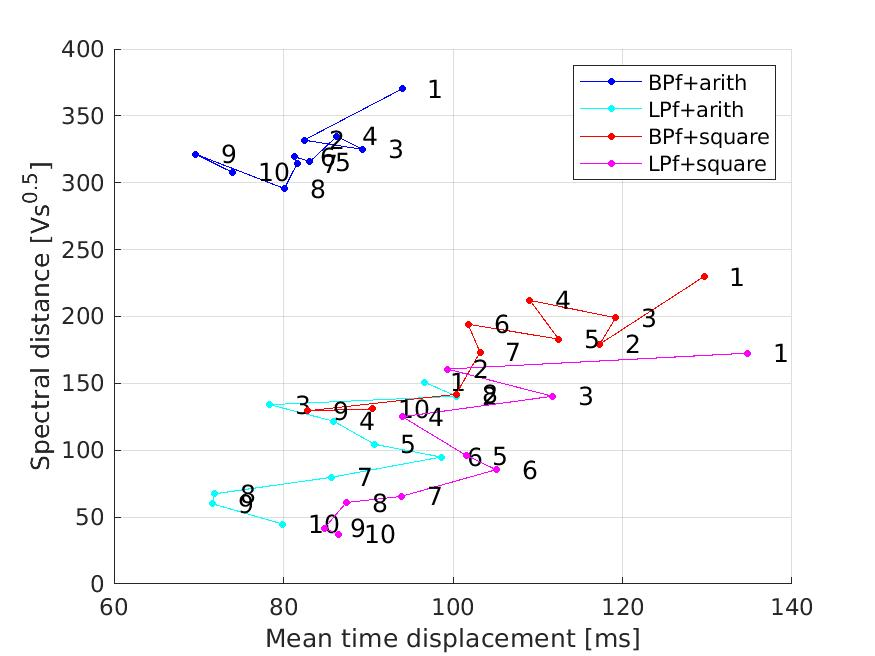
\includegraphics[width=1\linewidth]{results/scatter2.jpg}
\caption{Impulso gaussiano. $SNR= \{1, ..., 10\}dB$}
\label{fig:scatter2}
\end{figure}


Nel grafico \ref{fig:scatter4} la correlazione positiva tra le metriche; trattandosi di un impulso a media nulla con una prima parte positiva e una seconda negativa, gli algoritmi a media quadratica vengono penalizzati per l'effetto che inducono sulla parte bassa dello spettro a causa della rumorosità.
Evidenza inattesa, il filtro passa banda porta anche in questo caso ad una minor capacità previsiva.

\begin{figure}[htbp]
\centering
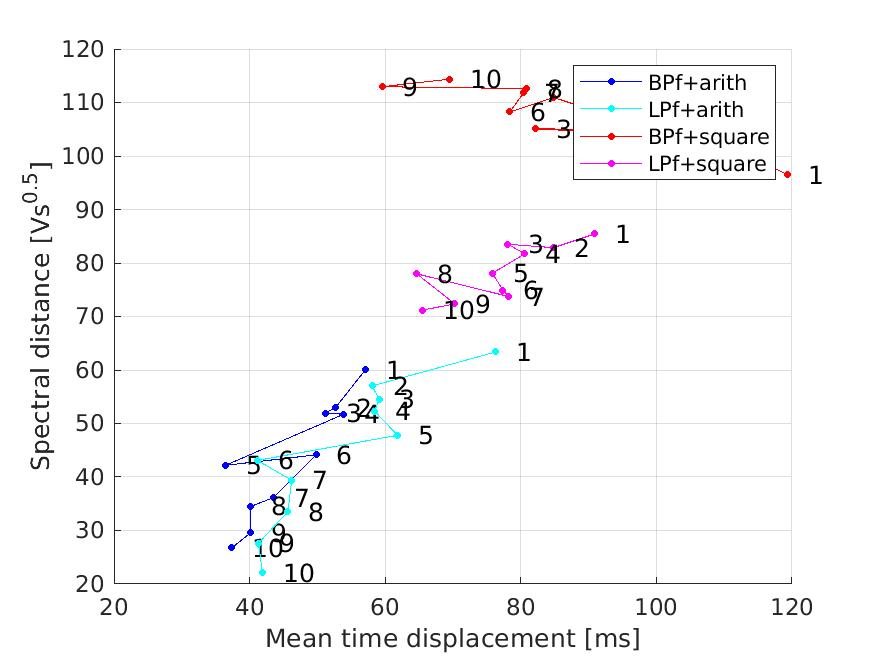
\includegraphics[width=1\linewidth]{results/scatter4.jpg}
\caption{Impulso spike. $SNR= \{1, ..., 10\}dB$}
\label{fig:scatter4}
\end{figure}

Nel caso dell'impulso sinusoidale il grafico \ref{fig:scatter5} conferma i risultati dell'impulso spike analogo.
PEr questo tipo di impilso si evidenzia una circostanza interessante con riguardo al test a media quadratica con filtro passa banda. A parità di aderenza dello spettro, la capacità previsiva si riduce drasticamente al decrescere del $SNR$.

\begin{figure}[htbp]
\centering
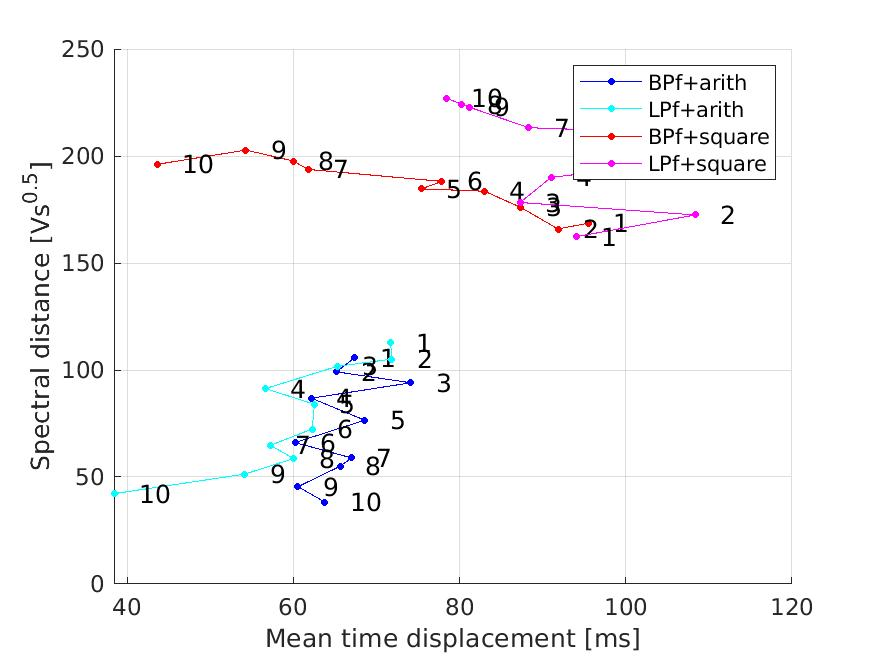
\includegraphics[width=1\linewidth]{results/scatter5.jpg}
\caption{Impulso sinusoidale. $SNR= \{1, ..., 10\}dB$}
\label{fig:scatter5}
\end{figure}


\section{Conclusioni}
\label{conclusioni}

In tutti i casi considerati, al variare del $SNR$ e della forma dell'impulso, il test che garantisce miglior capacità previsiva e aderenza degli spettri del segnale e del segnale filtrato è quello a media aritmetica accoppiato ad un filtro passa basso.

\subsection{Filtro LP vs BP}
Il filtro passa banda risulta problematico a causa dell'arbitraria forma che induce sugli spettri, tendendo a rendere il test poco robusto e adattabile alla forma dell'impulso. In un contesto sperimentale in cui la forma degli impulsi non è nota questo può risultare in scarse abilità previsive dell'algoritmo.

\subsection{Media semplice vs quadratica}
Gli algoritmi a media quadratica distorgono gli spettri del segnale filtrato in due modi: (1) aumentano le basse frequenze proporzionalmente al rumore del segnale; (2) allargano i picchi caratteristici della forma d'impulso considerata.

Se ad un prima analisi il primo effetto porta ad una migliore aderenza degli spettri per gli impulsi a media positiva (rettangolare o gaussiano), si verifica invece che sotto il profilo temporale la capacità previsiva si riduce. La miglior aderenza degli spettri nella parte bassa dello spettro è infatti dovuta a densità spettrale rumorosa e non di segnale.


\section{Riferimenti bibliografici}

% Full references (to aid the editor and reviewers) must be included. This will be produced automatically if you are using a .bib file.

% \bigskip
% \noindent Add citations manually or use BibTeX. See \cite{Chitimalla:17,Wen:16}.

% Bibliography
\bibliography{biblio/biblio.bib}

%Manual citation list
%\begin{thebibliography}{1}
%\bibitem{Zhang:14}
%Y.~Zhang, S.~Qiao, L.~Sun, Q.~W. Shi, W.~Huang, %L.~Li, and Z.~Yang,
 % \enquote{Photoinduced active terahertz metamaterials with nanostructured
  %vanadium dioxide film deposited by sol-gel method,} Opt. Express \textbf{22},
  %11070--11078 (2014).
%\end{thebibliography}




% JOCN authors may include their biographies and photos. This section is not required 

% \section*{Author Biographies}
% 
% \setlength\intextsep{0pt}
% 

% \paragraph{}
% \noindent \textbf{First A. Author} (M’76–SM’81–F’87) and the other authors may include biographies at the end of regular papers. This author became a Member (M) of IEEE in 1976, a Senior Member (SM) in 1981, and a Fellow (F) in 1987. The first paragraph may contain a place and/or date of birth (list place, then date). Next, the author’s educational background is listed. The degrees should be listed with type of degree in what field, which institution, city, state, and country, and year degree was earned. The author’s major field of study should be lower-cased.
  


% \begin{wrapfigure}{L}{0.21\textwidth}
%      \includegraphics[width=0.2\textwidth]{alicesmith}
%    \end{wrapfigure}
%    \noindent
%    \textbf{Alice Smith} received her BSc (Mathematics) in 2000 from The University of Maryland. Her research interests also include lasers and optics.\\
  
  

  
\pagebreak

% \section{Appendix}
% 
% 
% \subsection{Densità spettrali}
% 
% 
% \begin{figure}[htbp]
% \centering
% \fbox{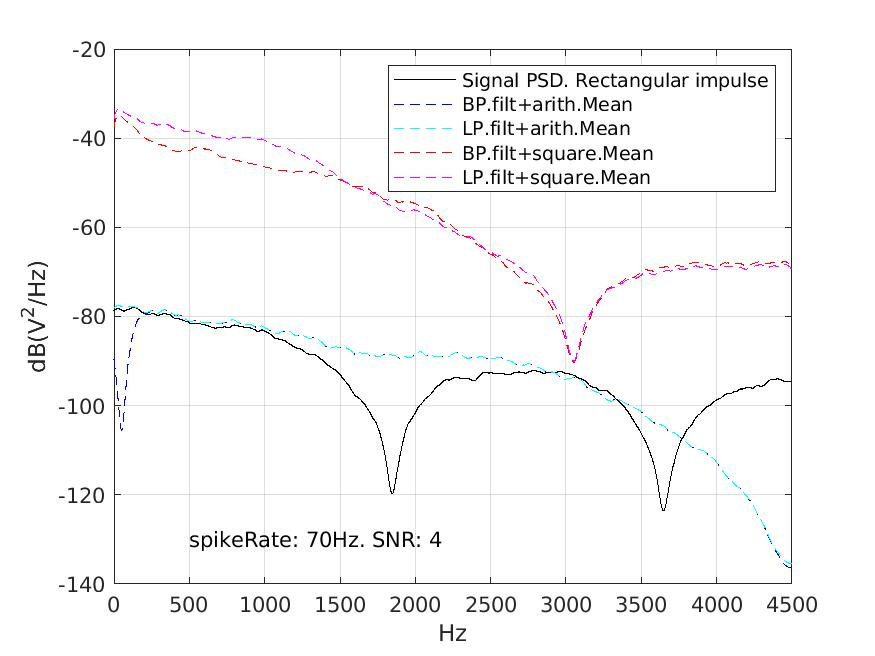
\includegraphics[width=1\linewidth]{results/c9_I1SNR4spec.jpg}}
% \caption{Spectral density of signal and filtered signal.}
% \label{fig:c9_I1SNR4spec}
% \end{figure}
% 
% \begin{figure}[htbp]
% \centering
% \fbox{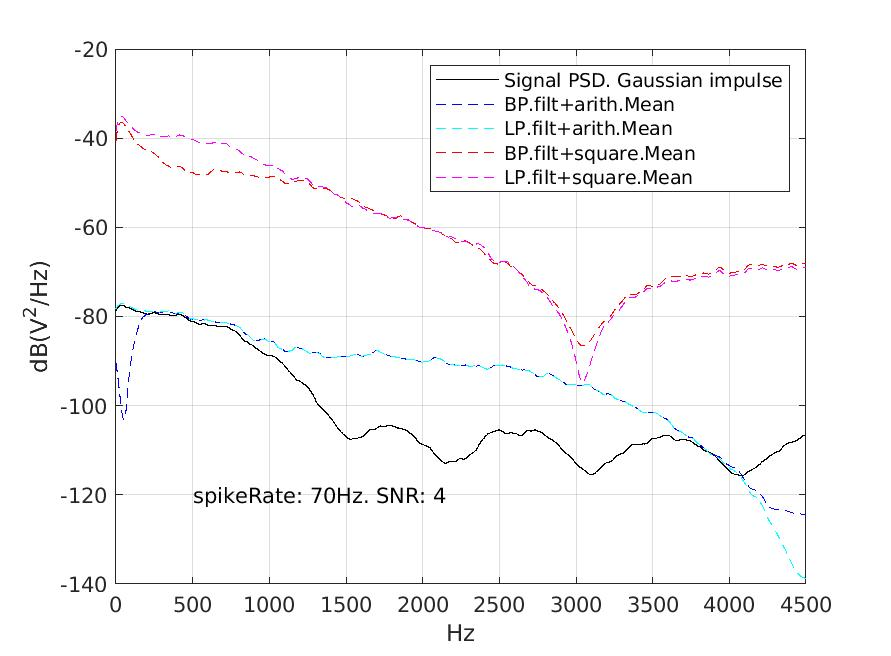
\includegraphics[width=1\linewidth]{results/c9_I2SNR4spec.jpg}}
% \caption{Spectral density of signal and filtered signal.}
% \label{fig:c9_I2SNR4spec}
% \end{figure}
% 
% \begin{figure}[htbp]
% \centering
% \fbox{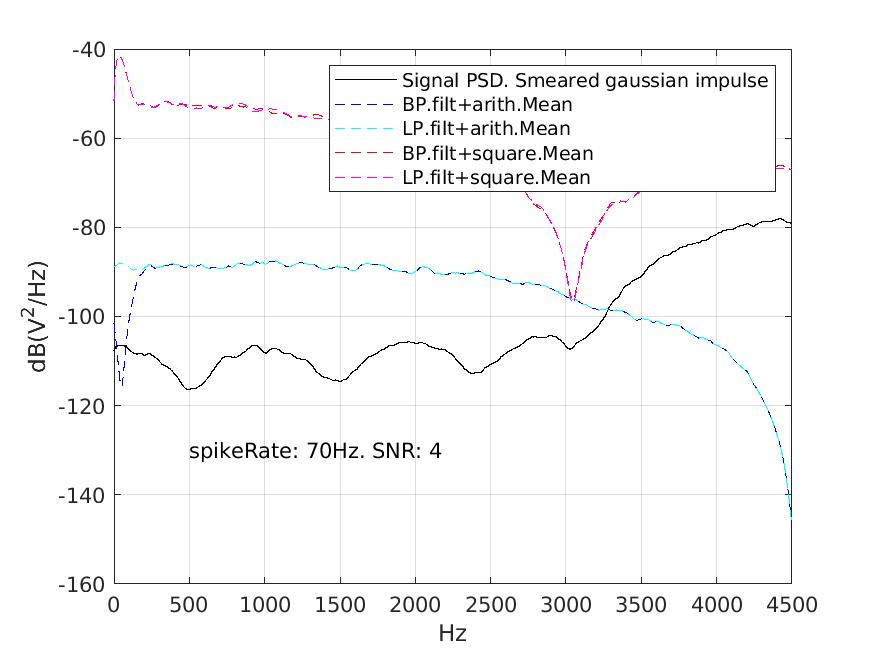
\includegraphics[width=1\linewidth]{results/c9_I3SNR4spec.jpg}}
% \caption{Spectral density of signal and filtered signal.}
% \label{fig:c9_I3SNR4spec}
% \end{figure}
% 
% \begin{figure}[htbp]
% \centering
% \fbox{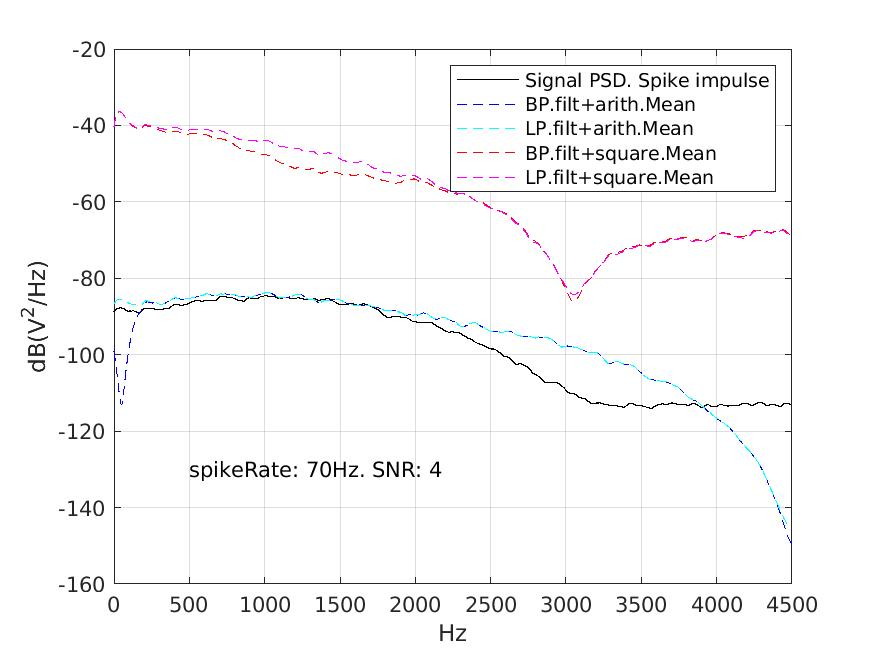
\includegraphics[width=1\linewidth]{results/c9_I4SNR4spec.jpg}}
% \caption{Spectral density of signal and filtered signal.}
% \label{fig:c9_I4SNR4spec}
% \end{figure}
% 
% \begin{figure}[htbp]
% \centering
% \fbox{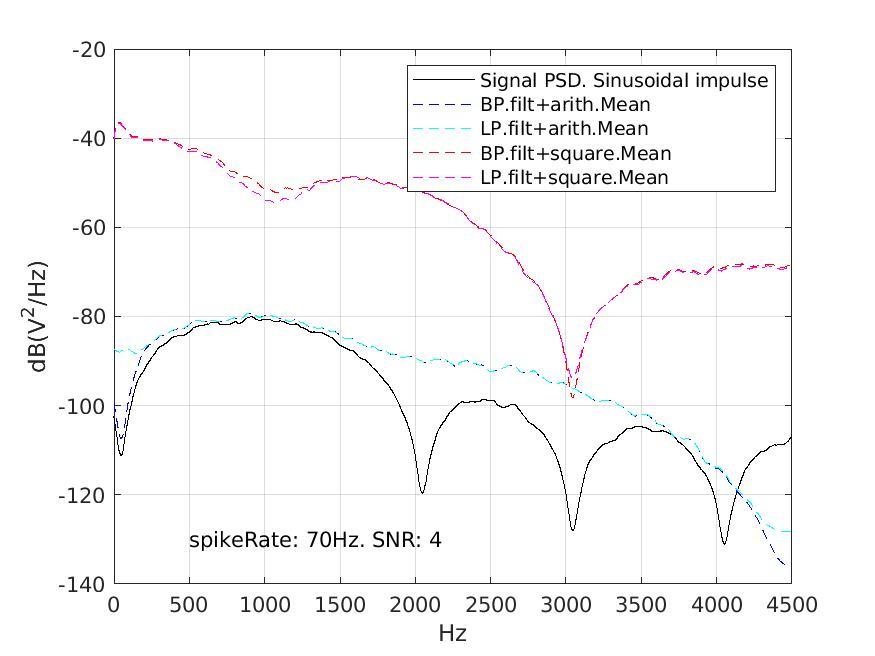
\includegraphics[width=1\linewidth]{results/c9_I5SNR4spec.jpg}}
% \caption{Spectral density of signal and filtered signal.}
% \label{fig:c9_I5SNR4spec}
% \end{figure}
% 
% 
% 
% \subsection{Distribuzione congiunta metriche}
% 
% 
% \begin{figure}[htbp]
% \centering
% \fbox{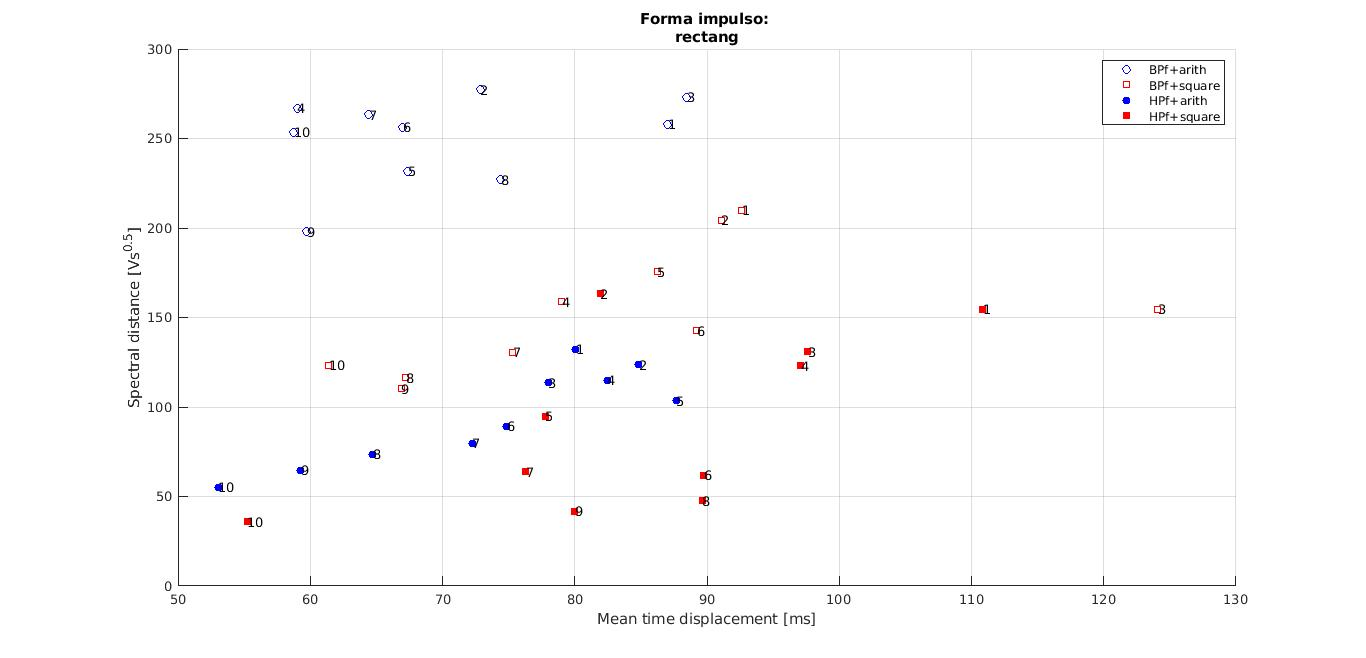
\includegraphics[width=.8\linewidth]{results/rectaScatter.jpg}}
% \caption{Impulso rettangolare. Metriche di valutazione.}
% \label{fig:rectaScatter}
% \end{figure}
% 
% \begin{figure}[htbp]
% \centering
% \fbox{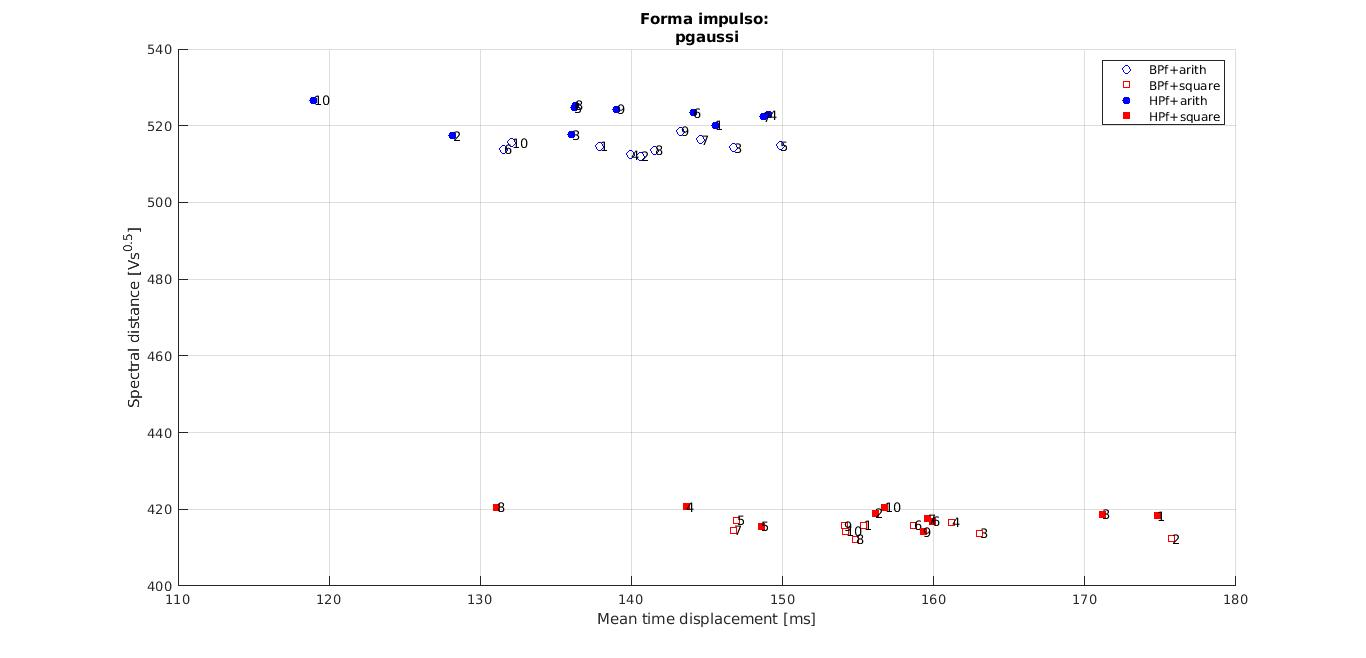
\includegraphics[width=.8\linewidth]{results/pgaussScatter.jpg}}
% \caption{Impulso gaussiano sfasato. Metriche di valutazione.}
% \label{fig:pgaussScatter}
% \end{figure}
% 
% \begin{figure}[htbp]
% \centering
% \fbox{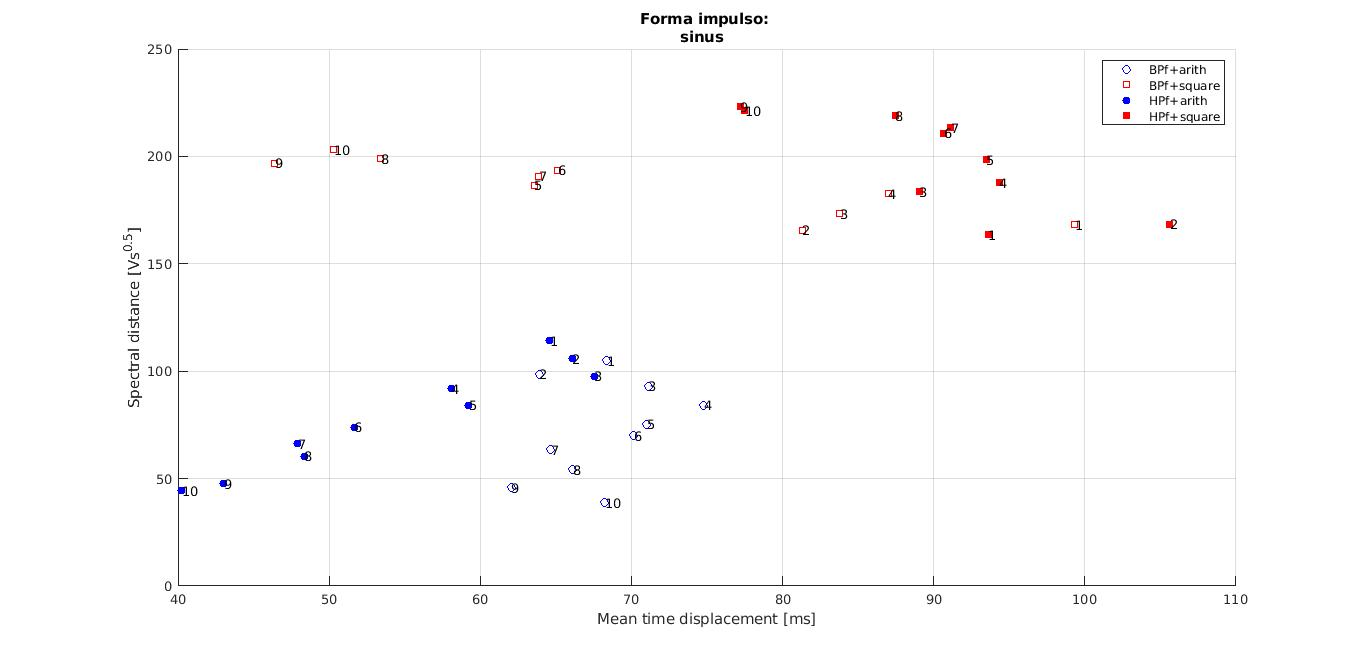
\includegraphics[width=.8\linewidth]{results/sinusScatter.jpg}}
% \caption{Impulso sinusoidale. Metriche di valutazione.}
% \label{fig:sinusScatter}
% \end{figure}


\end{document}




% \begin{algorithm}
% \caption{Euclid’s algorithm}\label{alg:euclid}
% \begin{algorithmic}[1]
% \Procedure{Euclid}{$a,b$}\Comment{The g.c.d. of a and b}
% \State $r\gets a\bmod b$
% \While{$r\not=0$}\Comment{We have the answer if r is 0}
% \State $a\gets b$
% \State $b\gets r$
% \State $r\gets a\bmod b$
% \EndWhile\label{euclidendwhile}
% \State \textbf{return} $b$\Comment{The gcd is b}
% \EndProcedure
% \end{algorithmic}
% \end{algorithm}
